\chapter{Vision}
This chapter covers the component for transforming 2D stereo images into 3D point clouds useful for reconstruction. The input sensor is a a stereo camera interfaced through ROS. The description covers the camera calibration process, the preprocessing of images, the inference of depth data and the generation of point clouds.

\section{Theory - Dense Stereo}

Dense stereo uses two 2D images and converts them to a dense 3D point cloud. That is the 3D position of every point in the 2D images is desired. To obtain this the disparity between all features are required, and the following stages are done with that in mind. The stages are as following.

\begin{itemize}
  \item Undistortion
  \item Rectification
  \item Correspondence
  \item Reprojection
\end{itemize}


\subsection{Preprocessing}
The undistortion and rectification processes are performed automatically and therefore only a short description will be included. The purpose of preprocessing is to transform the images, since this is more effective than making the functions take the parameters into account.

Because a lens is used for the cameras the pin hole model where a 3D point, X, is mapped to the image plane, x, by $ x = f X/Z $, where f is the focal length and Z is the distance to the camera, cannot be used. Both radial and tangential distortion exist respectively creating circular and elliptical distortion. By correcting the image for these parameters all pixels now follow the camera model and their projection line can be found.

The basic idea of rectification is to align epipolar lines in the two images, thus making them coplanar, thus reducing the search for corresponding pixels from 2D to 1D. Since the transform between the two cameras is known from calibration, this can be done with a linear transformation.

%Leon removed: The basic idea of rectification is based on epipolar lines. Epipolar lines are created by knowing the transform between the cameras. For every single point in one camera the line on which it can appear on another camera can be found. That is the epipolar line is a mapping of a pixels projection line in one camera onto the image plane of another camera. 
%
%By knowing the transformation between the two images, epipolar lines can be created for every point. An epipolar line is the line on which any point in one image must be positioned in the other image. Thus making the search for a feature much faster as it only occurs in one dimension.
%
%Rectification takes this one step further. By rectifying the two images the camera planes are angled towards the baseline, thus being parallel. Making the search for correspondence a 1D horizontal task, drastically increasing the speed.

Thus undistortion is a manipulation done independently for the cameras and the rectification is performed for the two cameras together, using respectively the intrinsic and extrinsic parameters.


\subsection{Correspondence} \label{sec:correspondence}
In dense stereo vision triangulation based on epipolar geometry is used to infer depth in the image. To do this each pixel in one image has to be matched to the corresponding pixel in the other image. This creates a disparity map for all pixels in the images. Though there is no guarantee that the disparity map is actually correct. The main goal in dense stereo can be described as minimizing the global error. 

Most of the top-ranked algorithms for the Middlesbury Stereo vision comparison use global optimization \cite{Hirschmuller2008}. Global optimization tries to minimize the overall error in the disparity image, i.e. creating the optimal disparity image. As this is an NP-hard problem and this application must run online, those were not considered.

The opposite approach is a horizontal 1D scan. As the rectification of the images guarantees horizontal epipolar lines, the most simple approach would be a 1D scan optimized for the lowest error. The problem is that a single scan line algorithm would lead to a very low vertical consistency of disparity. Instead a Semi-Global Block Matching algorithm (SGBM) is used as a compromise between the two methods. 

The idea of the semi global matching is an optimization of the disparity locally, but consistent. Following equation \ref{eq:cost} the penalty for small changes and large changes are distinguished as respectively $P_{1}$ and $P_{2}$. Here C is the pixel-wise matching cost for disparity $D_{\textbf{p}}$ at position \textbf{p} and \textbf{q} is nearby positions.

\begin{equation}\label{eq:cost}
\begin{split}
E(D) = \sum\limits_{\textbf{p}}(C(\textbf{p},D_{\textbf{p}}) + \sum\limits_{\textbf{q} \in N_{\textbf{p}} } P_{1} T [|D_{\textbf{p}} - D_{\textbf{q}}| = 1] + \sum\limits_{\textbf{q} \in N_{\textbf{p}} } P_{2} T [|D_{\textbf{p}} - D_{\textbf{q}}| > 1]
\end{split}
\end{equation} 

The optimization is then done as a shortest path for multiple 1D paths. Figure \ref{fig:paths} shows an example of this using 16 paths, in the actual implementation only 5 paths are used to optimize for speed. A disparity range for which the path is found is defined beforehand, thus a limit is set to which disparities can be found. 

\marginnote{needs reference}
\begin{figure}[h!]
  \centering
    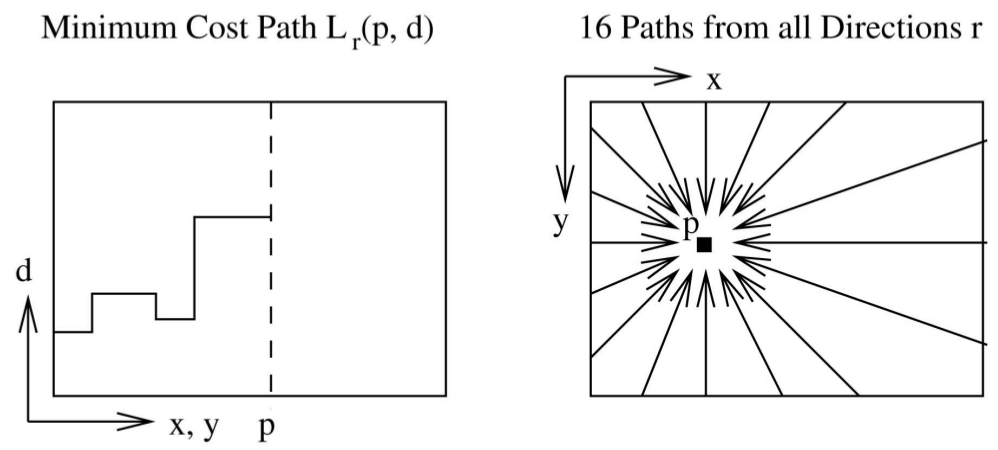
\includegraphics[scale=0.2]{graphics/06_vision/cost_aggregation.jpg}
      \caption{Costs for all directions are calculated using specific disparities and the disparity with the shortest path is found.}
    \label{fig:paths}
\end{figure}

Mutual information \cite{egnal2000mutual} is used as the pixel-wise matching. Using mutual information makes the algorithm much better at handling handling radiometric distances. The mutual information needs the disparity map to calculate the pixel matching cost, $ C_{MI} $ because the algorithm starts with a downscaled disparity guess and consistently runs through and upscales until it reaches full size. 

Consistency check is performed as in equation \ref{eq:consistency} using both disparity images. This removes errors that were created by occlusions in any of the images. Thus if the disparities differ they are set to invalid. 

%\begin{equation}\label{eq:consistency}
%D_{p} =  
%\left{\begin{matrix}
%D_{bp}	&  if|D_{bp} - D_{mq}| \leq 1, \\
%D_{inv} & otherwise
%\end{matrix}\right.
%\end{equation} 

\begin{equation} \label{eq:consistency}
D_{p} =
\left\{\begin{matrix}
D_{bp}	&  if|D_{bp} - D_{mq}| \leq 1, \\
D_{inv} & otherwise
\end{matrix}\right.
\end{equation}\\ 

%\begin{equation}\label{eq:qdefinition}
% \begin{split}
%  q = e_{bm}(p,D_{bp}) 
% \end{split}
%\end{equation} 

The flowchart of the complete system as described in the original article \cite{Hirschmuller2008} can be seen in figure \ref{fig:complete_system}.


\begin{figure}[h!]
  \centering
    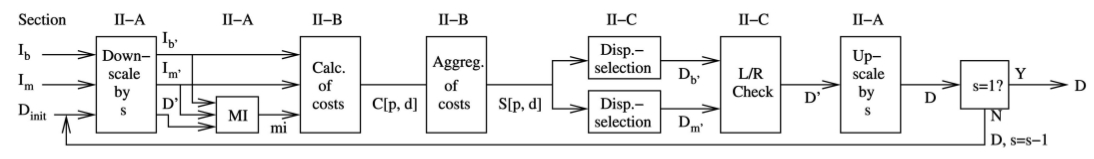
\includegraphics[width=\textwidth]{graphics/06_vision/complete_system.jpg}
     \caption{ Flowchart of the complete stereo process for SGBM. } 
    \label{fig:complete_system}
\end{figure}


\subsection{Reprojection} \label{sec:reprojection}

During the calibration of the cameras, projection matrices were obtained for both cameras. The projection matrices are based on the left camera lens, meaning the baseline, distance to the left camera, is 0 for the left matrix. By multiplying the projection matrix with a 3D point in the left cameras coordinate system, the points position in the image can be found as in equation \ref{eq:projection}. 


\begin{equation}\label{eq:projection}
 \begin{split}
  \begin{pmatrix}
   x \\
   y \\
   \omega 
  \end{pmatrix}	
  = 
  \begin{pmatrix}
    F_{x} & 0 & C_{x} & -F_{x}T_{x} \\
    0 & F_{y} & C_{y} & 0 \\
    0 & 0 & 1 & 0
  \end{pmatrix}
  \begin{pmatrix}
   X \\
   Y \\
   Z \\
   1 
  \end{pmatrix}	
 \end{split}
\end{equation}  


Here $F_{x}$ and $F_{y}$ are the focal length of the camera, $C_{x}$ and $C_{y}$ are the middle position of the image.

$T_{x}$ is the translation to the left camera. That is for the right camera it is the baseline and for the left it is 0. The baseline is measured in millimetres. 

But the goal is to obtain the opposite, the transform from 2D to 3D. That is the action of converting the obtained disparity map into a 3D point cloud. To do that the x and y positions are combined with the disparity. Thus multiplying with the Q matrix the 3D map position can be found.

\[ Q [ x \ y \ d \ 1 ]^{T} = [ X \ Y \ Z \ W ]^{T} \]

Where the Q matrix is defined by the parameters in the right projection matrix, except for the $C_{x}'$.

\[
Q =
 \begin{pmatrix}
  1 & 0 & 0 & -C_{x} \\
  0 & 1 & 0 & -C_{y} \\
  0 & 0 & 0 & F_{x} \\
  0 & 0 & -1/T_{x} & (C_{x}-C_{x}')/T_{x} 
 \end{pmatrix}
\]

Thus multiplying with the above mentioned vector, and scaling W to one the 3D position can be obtained.

\[
 \begin{pmatrix}
  x - C_{x} \\
  y - C_{y} \\
  F_{x} \\
  d-1/T_{x} 
 \end{pmatrix}
 \Rightarrow
  \begin{pmatrix}  
  X\\
  Y\\
  Z
 \end{pmatrix}
 =
 \begin{pmatrix}
  \dfrac{x - C_{x}}{ d(-1/T_{x})}  \\
  \dfrac{y - C_{y} }{ d(-1/T_{x})}\\
  \dfrac{F_{x}}{ d(-1/T_{x})}\\
  1
 \end{pmatrix}
\]

\section{Method - Images to point cloud}

As the project uses ROS for communication between nodes as much as possible of the stereo operations has been implemented within this framework, although not always possible as explained in \ref{sec:optimizing_parameters}. In the following the implementations will be described and evaluated.

\subsection{Calibration} \label{sec:calibration}

To perform the undistortion and rectification the intrinsic and extrinsic parameters of the cameras are required. These were obtained by the ROS node stereo\_camera\_calibrate by capturing images of a known chessboard pattern in different positions and rotations. When enough images have been captured the ROS node can solve for the camera parameters. It thus returns the camera matrix along with distortion parameters and the distance between the cameras. A small calibration plate was used, so that the calibration could be done within one meter of camera, fitting the parameters for the specific task.

\subsection{Undistortion and rectification}

Undistortion and rectification is done with a simple ROS node $image\_proc$. By giving the raw images together with a camera calibration file, created beforehand in section \ref{sec:calibration}. It uses these and returns rectified and undistorted images ready to be used by block matching algorithms.

\subsection{Block matching and reprojection}

The block matching is done with the OpenCV function createStereoSGBM \cite{opencv} described in section \ref{sec:correspondence}. Time stamps are checked on the images to make sure that they are recorded at the same time. The SGBM then uses the images and a set of parameters to make a disparity map. As most of these parameters are application specific they are discussed in section \ref{sec:optimizing_parameters}. 

%Conversion from int16 to float32 by division of 16.
Block matching and reprojection are implemented in a ROS node taking the rectified images as input, creating the disparity map and reprojection based on the openCV function.
 
\section{Evaluation}
Here results from the different operations are shown, these results are qualitative to show that the concept works not quantitative for a measurement of how well.

\subsection{Calibration}
From the calibration both the distortion, rectification and projection matrices are returned. The distortion parameters can be seen in equation \ref{eq:distortion}. A more in depth description of the undistorion can be seen in the OpenCV book \cite{locv}.

\begin{equation}\label{eq:distortion}
\begin{split}
[ k_{1}, k_{2}, p_{1}, p_{2}, k_{3} ] = [\ -0.422868,\ 0.192589,\ -0.000004,\ 0.002985,\ 0.000000\ ]
\end{split}
\end{equation} 

The rotation matrix for rectification is also returned from the calibration. From equation \ref{eq:rectification} it can be seen that the rotation needed is small, but it is still needed for the 1D correspondence search to work. 

\begin{equation}\label{eq:rectification}
\begin{split}
R =
 \begin{pmatrix}
  0.998701 & -0.002701 & -0.050892 \\
  0.002645 & 0.999996 & -0.001179 \\
  0.050895 & 0.001043 & 0.998703 
 \end{pmatrix}
\end{split}
\end{equation}

Figure \ref{fig:rectified} shows an example of two output images from $image\_proc$. The images have been undistorted and rectified by the function and horizontal lines have been included to demonstrate the alignment of the images, thus showing the effectiveness of the image to align features.

\begin{figure}[h!]
  \centering
    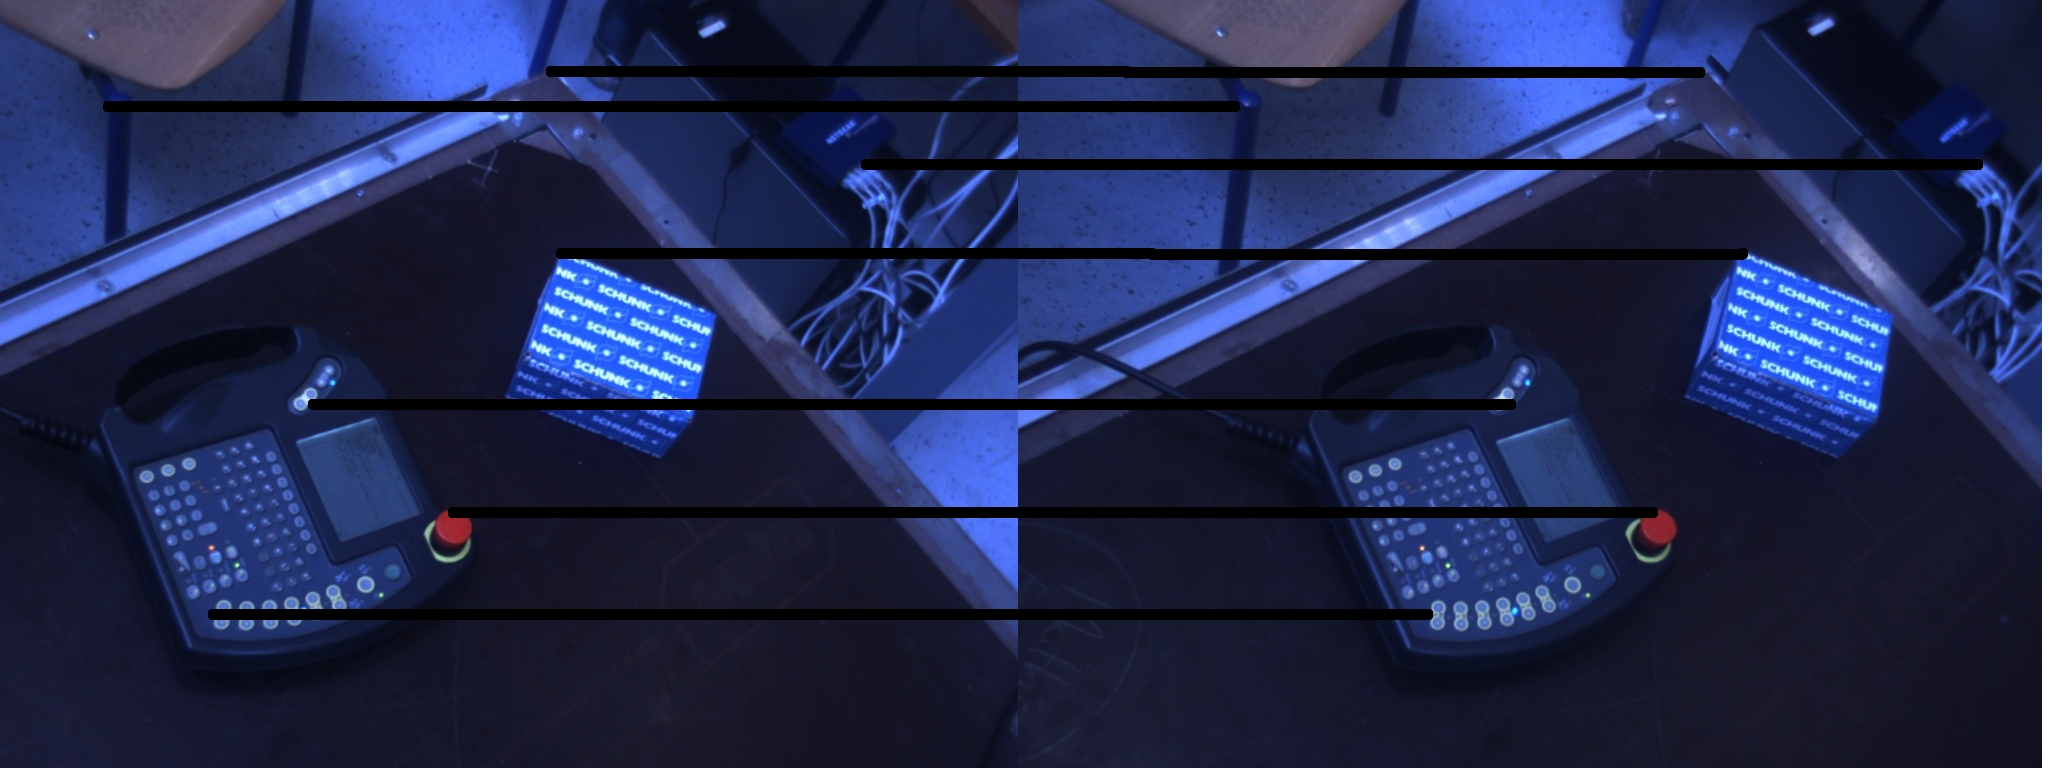
\includegraphics[width=\textwidth]{graphics/06_vision/rectified.jpg}
      \caption{Result of undistortion and rectification on an image pair. The horizontal lines shows corresponding pixels in the two images.}
    \label{fig:rectified}
\end{figure}

\subsection{Disparity map}

From two rectified images the disparity map can be created. Figure \ref{fig:disparity} is an example of such. The overall structure of the scene is recognizable, but it can be seen that algorithm does not necessarily guarantees complete coverage with standard parameters. In section \ref{sec:optimizing_parameters} a discussion of the selection of those parameters is included.

\begin{figure}[h!]
   \centering
    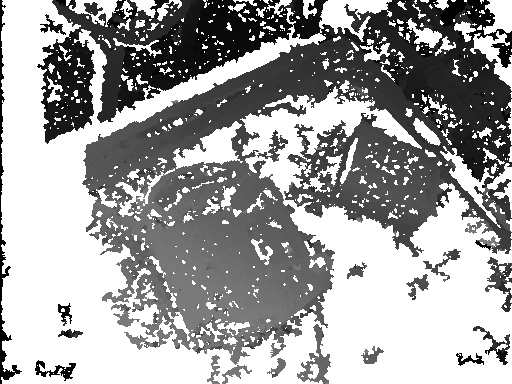
\includegraphics[scale=0.4]{graphics/06_vision/disparity_example.jpg}
    \caption{Disparity image for the two images shown in figure \ref{fig:rectified}. }
    \label{fig:disparity}
\end{figure}


\subsection{Reprojected point clouds} \label{sec:repro_point}

The only thing left to do is reprojecting the disparity map into 3D coordinates. From the calibration the parameters in \ref{eq:parameters} were given for the right camera.

\begin{equation}\label{eq:parameters}
\begin{split}
C_{x} = 582.152313 \\
C_{y} = 393.397633 \\
F_{x} = 1321.556521 \\
-F_{x}T_{x} = 158.751707 
\end{split}
\end{equation} 

Given $ -F_{x}T_{x} $ the baseline between the cameras calculated as in equation \ref{eq:baseline}.

\begin{equation}\label{eq:baseline}
\begin{split}
Tx = -F_{x}T_{x}/(-Fx) = Tx = 158.8/-1321.6 = 0.1201 meters
\end{split}
\end{equation} 

Using these parameters for the Q-matrix, the disparity image is reprojected to 3D. An example of the reprojection for the disparity image in figure \ref{fig:disparity} can be seen in figure \ref{fig:point_repro}


\begin{figure}[h!]
  \centering
    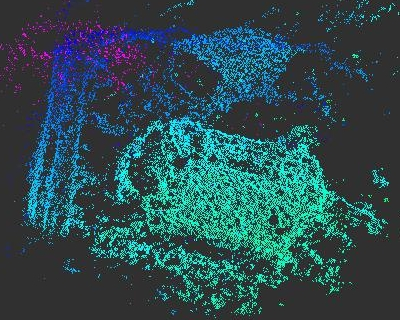
\includegraphics[scale=0.7]{graphics/06_vision/point_cloud_example2.jpg} %trim=l b r t
  \caption{Point cloud reprojected using the parameters shown in section \ref{sec:repro_point} performed on the disparity image in figure \ref{fig:disparity}. }
    \label{fig:point_repro}
\end{figure}


\section{Optimizing parameters towards the task } \label{sec:optimizing_parameters}

In most of the functions the input were non-adjustable values, but for the SGBM there are certain parameters where no single answers exist. The most important being the disparity range i.e. how far the algorithm will search for disparities.


When the 3D positions were extracted in section \ref{sec:reprojection} the connection in equation \ref{eq:disp1} between distance and disparity were found.

\begin{equation}\label{eq:disp1}
\begin{split}
Z = \dfrac{F_{x}}{ d(-1/T_{x})}
\end{split}
\end{equation} 

When solving for disparity the connection in equation \ref{eq:disp2} is given.

\begin{equation}\label{eq:disp2}
\begin{split}
 d = \dfrac{F_{x}T_{x}}{ Z}
\end{split}
\end{equation} 

That is with a known distance to the set-up the search area is known and thus the disparity range can be calculated. The distance is approximately 0.5 meters and the focal length and baseline are known from the calibration as shown in section \ref{sec:repro_point}. Thus the expected disparity can be calculated as in equation \ref{eq:disp3}.

\begin{equation}\label{eq:disp3}
\begin{split}
d = \dfrac{1321.55 pixel*0.1201m}{0.5m} = 317.4 pixel
\end{split}
\end{equation}

The minimum and maximum disparity have to range around this number. It is because of this that the point cloud generated from the ROS $image\_proc$ cannot be used. The node is only able to search with a maximum disparity range of 128 pixel. This gives a minimum distance of 1.24 meters. This would not fit the desired set-up at all and therefore the automatically generated point cloud is rejected. The exact disparity range can be found by looking at the maximum size of the object. This is an important aspect as setting the correct disparity range will drastically improve the search time and potentially remove mismatches. The algorithm is only able to scale the disparity in ranges of 16.

From these equations the minimum and maximum disparity are respectively chosen to be $16*16=256$ and $16*24=384$, resulting in a range from $0.41$ to $0.61$ meters. Thus if the distance to object should move outside this range it will not be found.

Speckle settings are another important parameter. The speckle-size is the minimum size of a path for it not to be removed as noise and the speckle-range is how large the difference can be between neighbouring pixels for them to still be considered from the same path. Though adjusting this depends entirely on the use of the point cloud. If the reconstruction doesn't take care of noise the speckle-size should be very low. The speckle range should also accommodate the point cloud so as to keep the signal/noise as high as possible, but still fitting the system. 

